%\documentclass[compress,xcolor=table]{beamer}
\usepackage{etex}
%\documentclass{article}
%\usepackage{beamerarticle}
%\usepackage{pstricks,pst-node} % PSTricks package
\usepackage{tikz}
\usetikzlibrary{patterns,positioning,fit,arrows,matrix,calc,shapes.geometric,shapes.multipart,decorations.pathreplacing}
%\usepackage[turkish]{babel}
\usepackage[utf8]{inputenc}
\usepackage{listings}
\usepackage{multicol}
%\includeonlyframes{current}

\mode<article>
{
  \usepackage{fullpage}
  \usepackage{pgf}
  \usepackage{hyperref}
}

\mode<presentation>
{
  \usetheme{metuceng}

  %\setbeamercovered{transparent}
}


\title{Programming Languages}
\subtitle{Variables and Storage}
\author{Onur Tolga Şehitoğlu}
\institute[METU]{Computer Engineering}
\subject{Variables and Storage}
\date{}
	\titlegraphic{\insertmetutitle\insertlicense}


\begin{document}

\lstset{language=C,
        basicstyle=\scriptsize\ttfamily,
        keywordstyle=\color{blue!50!black}\bfseries,
        identifierstyle=\color{blue!60!green}\sffamily,
        stringstyle=\color{red!70!green}\ttfamily,
	commentstyle=\color{blue!30!white}\itshape,
        showstringspaces=true}
\setbeamercolor{hexample}{bg=green!5!white,fg=black}%
\setbeamercolor{cexample}{bg=blue!5!white,fg=black}%
\setbeamercolor{pexample}{bg=orange!5!white,fg=black}%
\setbeamercolor{oexample}{bg=violet!5!white,fg=black}%

 \frame[plain]{\maketitle}
 \begin{frame}
 \frametitle{Outline}
 \begin{multicols}{2}
 \small
 \tableofcontents
 \end{multicols}
 \end{frame}

\section{Storage}
\begin{frame}
\frametitle{Storage}
\begin{itemize}[<+->]
 \item Functional language  variables: math like, defined or solved. Remains same afterwards.
 \item Imperative language variables: variable has a state and value. It can be assigned to
 different values in same phrase.
 \item Two basic operations on a variable: \structure{inspect} and \structure{update}.
\end{itemize}
\end{frame}

\begin{frame}
Computer memory can be considered as a collection of \structure{cell}s.
\begin{columns}
 \begin{column}{.55\textwidth}
 \begin{itemize}[<+->]
  \item Cells are initially \structure{unallocated}.
  \item Then, \structure{allocated/undefined}. Ready to use but value unknown.
  \item Then, \structure{storable}
  \item After the including block terminates, again \structure{unallocated}
\end{itemize}
\end{column}
\begin{column}{.45\textwidth}\scriptsize \noindent
 \only<1-1>{
	\tikz \draw [pattern=crosshatch] (0,0) rectangle (0.6,1);}
% \psframebox[fillstyle=crosshatch]{\makebox[4em]{\rule{0pt}{2em}}}}
\only<2-2>{ 
	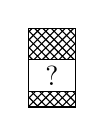
\begin{tikzpicture}
	\draw [pattern=crosshatch] (0,0) rectangle (0.6,1);
	\draw [fill=white] (0,0.2) rectangle (0.6,0.6);
	\node at (0.3,0.4) {?};
	\end{tikzpicture}}
%\psframebox[fillstyle=crosshatch]{\makebox[4em]{\rule{0pt}{2em}
%	\psframebox[fillstyle=solid,fillcolor=white]{x: ?}}}}
\only<3-3>{ 
	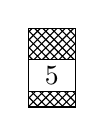
\begin{tikzpicture}
	\draw [pattern=crosshatch] (0,0) rectangle (0.6,1);
	\draw [fill=white] (0,0.2) rectangle (0.6,0.6);
	\node at (0.3,0.4) {5};
	\end{tikzpicture}}
%\psframebox[fillstyle=crosshatch]{\makebox[4em]{\rule{0pt}{2em}
%	\psframebox[fillstyle=solid,fillcolor=white]{x: 5}}}}
\only<4-4>{
	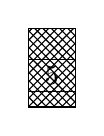
\begin{tikzpicture}
	\draw [pattern=crosshatch] (0,0) rectangle (0.6,1);
	\draw (0,0.2) rectangle (0.6,0.6);
	\node at (0.3,0.4) {5};
	\end{tikzpicture}}\\
%\psframebox[fillstyle=crosshatch]{\makebox[4em]{\rule{0pt}{2em}
%	\psframebox[fillstyle=none]{5}}}}\\
\texttt{
{\color<1-1>{red}{f();}}\\
void f() \{\\
{\color<2-2>{red}{\ \ \ int x;}}\\
\ \ \ ... \\
{\color<3-3>{red}{\ \ \ x=5;}}\\
\ \ \ ... \\
{\color<4-4>{red}{\ \ \ return;}}\\
\}
}
\end{column}
\end{columns}
\end{frame}

\defverbatim[colored]\codeupdateC{
\begin{lstlisting}[language={C}]
struct Complex { double x,y; } a, b;
...
a=b;                  // Total update
a.x=b.y*a.x;          // Selective update
\end{lstlisting}}

\begin{frame}
 \frametitle{Total or Selective Update}
\begin{itemize}
 \item Composite variables can be inspected and updated in total or selectively
 \item
\begin{beamercolorbox}{cexample}
 \codeupdateC
\end{beamercolorbox}
\item Primitive variables: single cell\\
	Composite variables: nested cells
\end{itemize}
\end{frame}

\subsection{Array Variables}
\begin{frame}
\frametitle{Array Variables}
Different approaches exist in implementation of array variables:
\begin{enumerate}
 \item Static arrays
 \item Dynamic arrays
 \item Flexible arrays
\end{enumerate}
\end{frame}

\defverbatim[colored]\codedizstatC{
\begin{lstlisting}[language={C}]
  #define MAXELS 100
  int a[10];
  double x[MAXELS*10][20];
\end{lstlisting}}
\begin{frame}
\frametitle{Static arrays}
\begin{itemize}
\item Array size is fixed at compile time to a constant value or expression.
\item C example:
\begin{beamercolorbox}{cexample}
\codedizstatC
\end{beamercolorbox}
\end{itemize}
\end{frame}

\defverbatim[colored]\codedizdinaC{
\begin{lstlisting}[language={C}]
int f(int n) {
    double a[n]; ...
}
\end{lstlisting}}
\defverbatim[colored]\codedizdinaCpp{
\begin{lstlisting}[language={C++}]
template<class T>  class Array {
      T *content;
  public:
      Array(int s) { content=new T[s]; }
      ~Array()     { delete [] content; }
};
...
Array<int>  a(10);             Array<double> b(n);
\end{lstlisting}}
\begin{frame}

\frametitle{Dynamic arrays}

\begin{itemize}
\item Array size is defined when variable is allocated. Remains constant afterwards.
\item Example: C90/GCC (not in ANSI)
\begin{beamercolorbox}{cexample}
\codedizdinaC
\end{beamercolorbox}
\item Example: C++ with \structure{templates}
\begin{beamercolorbox}{cexample}
\codedizdinaCpp
\end{beamercolorbox}

\end{itemize}
\end{frame}

\defverbatim[colored]\codedizesnekPerl{
\begin{lstlisting}[language={Perl}]
@a=(1,3,5);          # array size: 3 
print $#a , "\n";    # output: 2 (0..2)
$a[10] = 12;         # array size 11 (intermediate elements unknown)
$a[20] = 4;          # array size 21
print $#a , "\n";    # output: 20 (0..20)
delete $a[20];       # last  element erased,  size is 11
print $#a , "\n";    # output: 10 (0..10)
\end{lstlisting}
}
\begin{frame}
 \frametitle{Flexible arrays}
\begin{itemize}
 \item Array size is completely variable. Arrays may expand or shrink at run time.
	Script languages like Perl, PHP, Python
 \item Perl example:
\begin{beamercolorbox}{oexample}
\codedizesnekPerl
\end{beamercolorbox}
 \item C++ and object orient languages allow overload of \path{[ ]} operator to make flexible
 arrays possible. STL (Standard Template Library) classes in C++ like \structure{vector, map}
 are like such flexible array implementations.
\end{itemize}
\end{frame}

\section{Semantics of Assignment}
\begin{frame}
 \frametitle{Semantic of assignment in composite variables}
\begin{columns}
\begin{column}{.55\textwidth}
\begin{itemize}[<+->]
 \item Assignment by \structure{Copy} vs \structure{Reference}.
 \item \structure{Copy:} All content is copied into the other variables storage. Two copies
 with same values in memory.
 \item \structure{Reference:} Reference of variable is copied to other variable. Two variables
 share the same storage and values. 
\end{itemize}
\end{column}
\begin{column}{.45\textwidth}
\texttt{\tiny
 \only<2->{
 \begin{tabular}{|c|}
    \multicolumn{1}{l}{\tikz [remember picture] \node (x1) {\textsf{x}};} \\ 
    \multicolumn{1}{l}{\rule{0pt}{2pt}\tikz [remember picture] \node (xt1) {};} \\ \hline
    "ali" \\ \hline   55717 \\ \hline   3.56  \\ \hline
 \end{tabular} \tikz [remember picture, overlay] \draw [->,thick,blue] (x1) -- (xt1.south west);
 \begin{tabular}{|c|}
  \multicolumn{1}{l}{\tikz [remember picture] \node (y1) {\textsf{y}};} \\
  \multicolumn{1}{l}{\rule{0pt}{2pt}\tikz [remember picture] \node (yt1) {};} \\ \hline
   "veli" \\ \hline 123456 \\ \hline 2.48 \\ \hline
 \end{tabular}\tikz [remember picture,overlay] \draw [->,thick,blue] (y1) -- (yt1.south west);  \hfill\structure{\textsf{assignment by Copy:}}
\\[.5em]
\begin{tabular}{|c|}
    \multicolumn{1}{l}{\tikz [remember picture] \node (x2) {\textsf{x}};} \\ 
    \multicolumn{1}{l}{\rule{0pt}{2pt}\tikz [remember picture] \node (xt2) {};} \\ \hline
    "veli" \\ \hline   123456 \\ \hline   2.48  \\ \hline
 \end{tabular} \tikz [remember picture,overlay] \draw [->,thick,blue] (x2) -- (xt2.south west);
 \begin{tabular}{|c|}
  \multicolumn{1}{l}{\tikz [remember picture] \node (y2) {\textsf{y}};} \\
  \multicolumn{1}{l}{\rule{0pt}{2pt}\tikz [remember picture] \node (yt2) {};} \\ \hline
   "veli" \\ \hline 123456 \\ \hline 2.48 \\ \hline
 \end{tabular}\tikz [remember picture,overlay] \draw [->,thick,blue] (y2) -- (yt2.south west); }
%\tikz [remember picture,overlay] \draw [->,thick,blue] (once1) -- (sonra1); 
\only<3->{
\\[1em] \hrule
\begin{tabular}{|c|}
    \multicolumn{1}{l}{\tikz [remember picture] \node (x3) {\textsf{x}};} \\ 
    \multicolumn{1}{l}{\rule{0pt}{2pt}\tikz [remember picture] \node (xt3) {};} \\ \hline
    "ali" \\ \hline   55717 \\ \hline   3.56  \\ \hline
 \end{tabular} \tikz [remember picture,overlay] \draw [->,thick,blue] (x3) -- (xt3.south west); 
 \begin{tabular}{|c|}
  \multicolumn{1}{l}{\tikz [remember picture] \node (y3) {\textsf{y}};} \\
  \multicolumn{1}{l}{\rule{0pt}{2pt}\tikz [remember picture] \node (yt3) {};} \\ \hline
   "veli" \\ \hline 123456 \\ \hline 2.48 \\ \hline
 \end{tabular}\tikz [remember picture,overlay] \draw [->,thick,blue] (y3) -- (yt3.south west); \hfill\structure{\textsf{Assignment by reference:}}
\\[.5em]
 \begin{tabular}[t]{c}
  \multicolumn{1}{l}{\tikz [remember picture] \node (x4) {\textsf{x}};}\\
  \textrm{old}\\
  \textrm{value}\\
  \textrm{of \textsf{x}}\\
  \textrm{is lost}
 \end{tabular}
 \begin{tabular}[t]{|c|}
  \multicolumn{1}{l}{\tikz [remember picture] \node (y4) {\textsf{y}};} \\
  \multicolumn{1}{l}{\rule{0pt}{2pt}\tikz [remember picture] \node (yt4) {};} \\ \hline
   "veli" \\ \hline 123456 \\ \hline 2.48 \\ \hline
 \end{tabular}\tikz [remember picture,overlay] \draw [->,thick,blue] (y4) -- (yt4.south west);
	\tikz [remember picture, overlay] \draw [->,thick,blue] (x4) -- (yt4.south west);
}
}
\end{column}
\end{columns}
\end{frame}

\begin{frame}
 \begin{itemize}
  \item Assignment semantics is defined by the language design
  \item C structures follows copy semantics. Arrays cannot be assigned. Pointers are used to
  implement reference semantics. C++ objects are similar.
  \item Java follows copy semantics for  primitive types. All other types (objects) are
  reference semantics.
  \item Copy semantics is slower
  \item Reference semantics cause problems from storage sharing (all operations effect both
  variables). Deallocation of one makes the other invalid.
  \item Java provides copy semantic via a member function called \texttt{copy()}. 
  	Java garbage collector avoids invalid values (in case of deallocation)
 \end{itemize}
\end{frame}

\section{Variable Lifetime}
\begin{frame}
\frametitle{Variable Lifetime}
\begin{itemize}
 \item \structure{Variable lifetime:} The period between allocation of a variable and
 deallocation of a variable.
 \item 4 kinds of variable lifetime.
\begin{enumerate}
 \item Global lifetime (while program is running)
 \item Local lifetime (while declaring block is active)
 \item Heap lifetime (arbitrary)
 \item Persistent lifetime (continues after program terminates)
\end{enumerate}
\end{itemize}
\end{frame}

\subsection{Global Lifetime}
\begin{frame}
 \frametitle{Global lifetime}
\begin{itemize}[<+->]
 \item Life of global variables start at program startup and finishes when program terminates.
 \item In C, all variables not defined inside of a function (including \texttt{main()}) are
 global variables and have global lifetime:\\
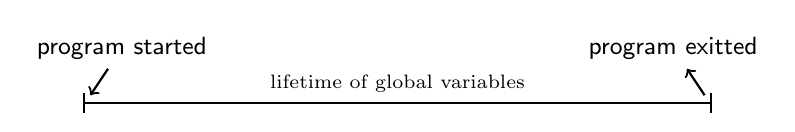
\begin{tikzpicture}
\node at (0.5,0.7) (ps) {\textsf{\small program started}};
\node at (7.5,0.7) (pe) {\textsf{\small program exitted}};
\draw [|-|,thick] (0,0) -- node[above,align=center] {\scriptsize lifetime of global variables}(8,0);
\draw [->,thick] (ps) -- (0.1,0.1);
\draw [<-,thick] (pe) -- (7.9,0.1);
\end{tikzpicture}
%\rnode{basla}{\textsf{\small program started}}\hfill
%	\rnode{bitis}{\textsf{\small program exitted}}\\
%\rnode{yarat}{}\hfill\rnode{bitir}{}
%\ncline[nodesep=4pt]{->}{basla}{yarat} \ncline[nodesep=4pt]{<-}{bitis}{bitir}
%\ncline{|-|}{yarat}{bitir}\lput{:U}{\tiny \rput(0,4pt){lifetime of global variables}}
\item What are \texttt{static} variables inside functions in C?
\end{itemize}
\end{frame}

\subsection{Local Lifetime}
\begin{frame}
 \frametitle{Local lifetime}
\begin{itemize}[<+->]
 \item Lifetime of a local variable, a variable defined in a function or statement block, is the
 time between the declaring block is activated and the block finishes.
 \item Formal parameters are local variables.
 \item Multiple instances of same local variable may be alive at the same time in recursive
 functions.
\item \ \\
{\tiny
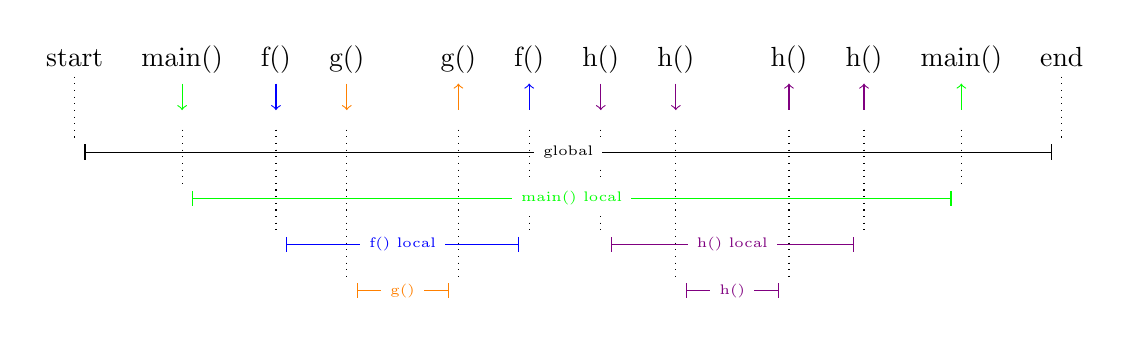
\begin{tikzpicture}[column sep=2.5mm]
\matrix (mat) [matrix of nodes,nodes in empty cells,ampersand replacement=\&] {
start \& main() \& f() \& g() \& \& g() \& f() \&   h()  \&   h()  \&  \&   h()  \&   h()  \&  main() \& end \\[1em]
      \&        \&     \&     \& \&     \&     \&        \&        \&  \&      \&        \&         \&     \\[0.5em]
      \&        \&     \&     \& \&     \&     \&        \&        \&  \&       \&        \&         \&     \\[1em]
      \&        \&     \&     \& \&     \&     \&        \&        \&  \&       \&        \&         \&     \\[1em]
      \&        \&     \&     \& \&     \&     \&        \&        \&  \&       \&        \&         \&     \\[1em]
      \&        \&     \&     \& \&     \&     \&        \&        \&  \&      \&        \&         \&     \\[1em]
};
\draw [dotted] (mat-1-1) -- (mat-3-1);
\draw [dotted] (mat-1-14) -- (mat-3-14);
\draw [->,green] (mat-1-2) -- (mat-2-2) ; \draw [dotted] (mat-2-2) -- (mat-4-2);
\draw [->,blue] (mat-1-3) -- (mat-2-3) ; \draw [dotted] (mat-2-3) -- (mat-5-3);
\draw [->,orange] (mat-1-4) -- (mat-2-4) ; \draw [dotted] (mat-2-4) -- (mat-6-4);
\draw [<-,orange] (mat-1-6) -- (mat-2-6) ; \draw [dotted] (mat-2-6) -- (mat-6-6);
\draw [<-,blue] (mat-1-7) -- (mat-2-7) ; \draw [dotted] (mat-2-7) -- (mat-5-7);
\draw [->,violet] (mat-1-8) -- (mat-2-8) ; \draw [dotted] (mat-2-8)--  (mat-5-8);
\draw [->,violet] (mat-1-9) -- (mat-2-9) ; \draw [dotted] (mat-2-9) -- (mat-6-9);
\draw [<-,violet] (mat-1-11) -- (mat-2-11) ; \draw [dotted] (mat-2-11) -- (mat-6-11);
\draw [<-,violet] (mat-1-12) -- (mat-2-12) ; \draw [dotted] (mat-2-12) -- (mat-5-12);
\draw [<-,green] (mat-1-13) -- (mat-2-13) ; \draw [dotted] (mat-2-13) -- (mat-4-13);
\draw [|-|] (mat-3-1) -- node [fill=white]  {\tiny global} (mat-3-14) ;
\draw [|-|,green] (mat-4-2) -- node [fill=white]  {\tiny main() local} (mat-4-13) ;
\draw [|-|,blue] (mat-5-3) -- node [fill=white]  {\tiny f() local} (mat-5-7) ;
\draw [|-|,orange] (mat-6-4) -- node [fill=white]  {\tiny g()} (mat-6-6) ;
\draw [|-|,violet] (mat-5-8) -- node [fill=white]  {\tiny h() local} (mat-5-12) ;
\draw [|-|,violet] (mat-6-9) -- node [fill=white]  {\tiny h()} (mat-6-11) ;
\end{tikzpicture}
}
\end{itemize}
\end{frame}
%\item {\tiny \psset{linewidth=.4pt,labelsep=0pt}
%\begin{tabular}[t]{llllrrllrrrr}
% \rnode[bl]{bb}{start} & \rnode[bl]{bm}{main()} & \rnode[bl]{bf}{f()} & 
%	\rnode[bl]{bg}{g()} & \rnode[br]{cg}{g()} & \rnode[br]{cf}{f()} & 
%	\rnode[bl]{bh1}{h()} & \rnode[bl]{bh2}{h()} & \rnode[br]{ch2}{h()} & 
%	\rnode[br]{ch1}{h()} & \rnode[br]{cm}{main()} & \rnode[br]{cb}{end} \\
%\rnode{dbb}{} & \rnode{dbm}{} & \rnode{dbf}{} & 
%	\rnode{dbg}{} & \rnode{dcg}{} & \rnode{dcf}{} & 
%	\rnode{dbh1}{} & \rnode{dbh2}{} & \rnode{dch2}{} & 
%	\rnode{dch1}{} & \rnode{dcm}{} & \rnode{dcb}{} \\
%\ncline{->}{bb}{dbb}
%\ncline[linecolor=green!40!black]{->}{bm}{dbm} 
%\ncline[linecolor=blue!60!black]{->}{bf}{dbf} 
%\ncline[linecolor=orange!60!black]{->}{bg}{dbg}  
%\ncline[linecolor=orange!60!black]{<-}{cg}{dcg}
%\ncline[linecolor=blue!60!black]{<-}{cf}{dcf} 
%\ncline[linecolor=violet]{->}{bh1}{dbh1} 
%\ncline[linecolor=violet!70!black]{->}{bh2}{dbh2}
%\ncline[linecolor=violet!70!black]{<-}{ch2}{dch2}
%\ncline[linecolor=violet]{<-}{ch1}{dch1} 
%\ncline[linecolor=green!40!black]{<-}{cm}{dcm}
%\ncline{<-}{cb}{dcb}
%\rnode{kb}{} & & & & & & & & & & & \rnode{kc}{} \\ 
%\ncline{|-|}{kb}{kc}\mput{\psframebox*{global}}
%  & \rnode{mb}{} & & & & & & & & & \rnode{mc}{} & \\ 
%\ncline[linecolor=green!40!black]{|-|}{mb}{mc}\mput{\psframebox*{main() local}}
%  &  & \rnode{fb}{} & & & \rnode{fc}{} & \rnode{h1b}{} & & & \rnode{h1c}{} & & \\ 
%\ncline[linecolor=blue!60!black]{|-|}{fb}{fc}\mput{\psframebox*{f() local}}
%\ncline[linecolor=violet]{|-|}{h1b}{h1c}\mput{\psframebox*{h() local}}
%  &  &  & \rnode{gb}{} & \rnode{gc}{} & &  & \rnode{h2b}{} & \rnode{h2c}{} & & & \\ 
%\ncline[linecolor=orange!60!black]{|-|}{gb}{gc}\Bput{g() local}
%\ncline[linecolor=violet!70!black]{|-|}{h2b}{h2c}\Bput{h() local}
%
%\end{tabular}
%}

\defverbatim[colored]\codeomurC{
\begin{lstlisting}[language={C},basicstyle=\tiny\ttfamily]
double x;
int h(int n) {
   int a;
   if (n<1) return 1
   else return h(n-1);
}
void g() {
   int x;
   int b;
...
}
int f() {
   double z;
   ...
   g();
   ...
}
int main() {
    double k;
    f();
    ...
    h(1);
    ...;
    return 0;
}
\end{lstlisting}}
\begin{frame}
\begin{columns}
\begin{column}{.5\linewidth}
 \begin{beamercolorbox}{cexample}
\codeomurC
 \end{beamercolorbox}
\end{column}
\begin{column}{.5\linewidth}
{\tiny
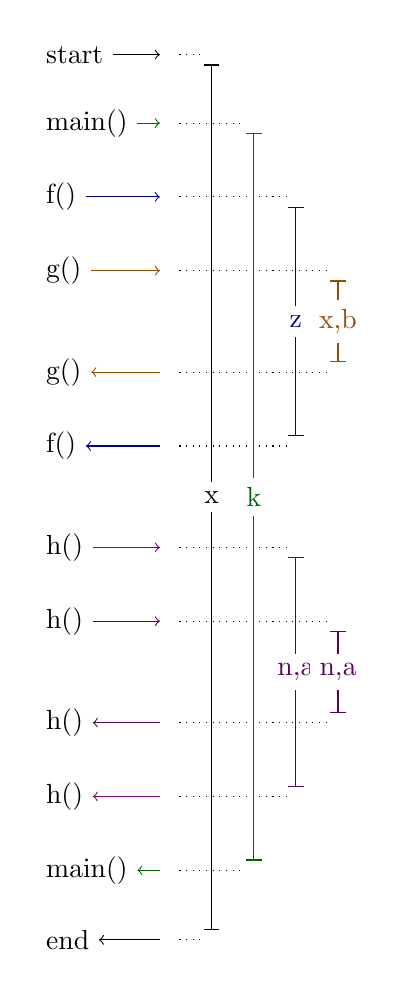
\begin{tikzpicture} 
\matrix [column sep=3mm,ampersand replacement=\&] {
\node [right](bb) {start}; \& \node (dbb) {}; \& \node (kb) {};  \\[1em]
\node [right](bm) {main()}; \& \node (dbm) {}; \&  \& \node (mb) {}; \\[1em]
\node [right](bf) {f()}; \& \node (dbf) {}; \&  \&  \& \node (fb) {}; \\[1em]
\node [right](bg) {g()}; \& \node (dbg) {}; \&  \&  \& \& \node (gb) {}; \\[2em]
\node [right](cg) {g()}; \& \node (dcg) {}; \&  \&  \& \& \node (gc) {}; \\[1em]
\node [right](cf) {f()}; \& \node (dcf) {}; \&  \&  \& \node (fc) {}; \\[2em]
\node [right](bh1) {h()}; \& \node (dbh1) {}; \&  \&  \& \node (h1b) {}; \\[1em]
\node [right](bh2) {h()}; \& \node (dbh2) {}; \&  \&  \& \& \node (h2b) {}; \\[2em]
\node [right](ch2) {h()}; \& \node (dch2) {}; \&  \&  \& \& \node (h2c) {}; \\[1em]
\node [right](ch1) {h()}; \& \node (dch1) {}; \&  \&  \& \node (h1c) {}; \\[1em]
\node [right](cm) {main()}; \& \node (dcm) {}; \&  \& \node (mc) {}; \\[1em]
\node [right](cb) {end}; \& \node (dcb) {}; \& \node (kc) {};  \\[1em]
};
\draw [->] (bb) -- (dbb);	\draw [dotted] (dbb) -- (kb);
\draw [green!40!black,->] (bm) -- (dbm);  		\draw [dotted] (dbm) -- (mb);
\draw [blue!60!black,->] (bf) -- (dbf);   		\draw [dotted] (dbf) -- (fb);
\draw [orange!60!black,->] (bg) -- (dbg);    		\draw [dotted] (dbg) -- (gb);
\draw [orange!60!black,<-] (cg) -- (dcg);  		\draw [dotted] (dcg) -- (gc);
\draw [blue!60!black,<-] (cf) -- (dcf);   		\draw [dotted] (dcf) -- (fc);
\draw [green!40!black,<-] (cm) -- (dcm);  		\draw [dotted] (dcm) -- (mc);
\draw [violet,->] (bh1) -- (dbh1);   		\draw [dotted] (dbh1) -- (h1b);
\draw [violet!70!black,->] (bh2) -- (dbh2);  		\draw [dotted] (dbh2) -- (h2b);
\draw [violet!70!black,<-] (ch2) -- (dch2);  		\draw [dotted] (dch2) -- (h2c);
\draw [violet,<-] (ch1) -- (dch1);   		\draw [dotted] (dch1) -- (h1c);
\draw [<-] (cb) -- (dcb);	\draw [dotted] (dcb) -- (kc);
\draw [|-|] (kb) -- node [fill=white] {x} (kc);
\draw [|-|,green!40!black] (mb) -- node [fill=white] {k} (mc);
\draw [|-|,blue!60!black] (fb) -- node [fill=white] {z} (fc);
\draw [|-|,orange!60!black] (gb) -- node [fill=white] {x,b} (gc);
\draw [|-|,violet!70!black] (h1b) -- node [fill=white] {n,a} (h1c);
\draw [|-|,violet!70!black] (h2b) -- node [fill=white] {n,a} (h2c);
\end{tikzpicture}
}
\end{column}
\end{columns}
\end{frame}




\subsection{Heap Variable Lifetime}
\begin{frame}
 \frametitle{Heap Variable Lifetime}
 \begin{itemize}[<+->]
  \item \structure{Heap variables:} Allocation and deallocation is not automatic but explicitly
  requested by programmer via function calls.
  \item C: \texttt{malloc(), free()}, C++: \texttt{new, delete}.
  \item Heap variables are accessed via pointers. Some languages use references\\
\texttt{\scriptsize double *p;\\
p=malloc(sizeof(double));\\
*p=3.4; ...\\
free(p);
}
  \item \alert{\texttt{p} and \texttt{*p} are different variables} \texttt{p} has pointer
  type and usually a local or global lifetime, \texttt{*p} is heap variable.
  \item heap variable lifetime can start or end at anytime.
 \end{itemize}
\end{frame}


\defverbatim[colored]\codeyiginC{
\begin{lstlisting}[language={C}]
double *p;
int h() { ...
}
void g() { ...
   p=malloc(sizeof(double));
}
int f() { ...
   g(); ...
}
int main() { ...
    f();    ...
    h();    ...;
    free(p); ...
}
\end{lstlisting}}
\begin{frame}
\begin{beamercolorbox}{cexample}
\codeyiginC
\end{beamercolorbox}
{\tiny
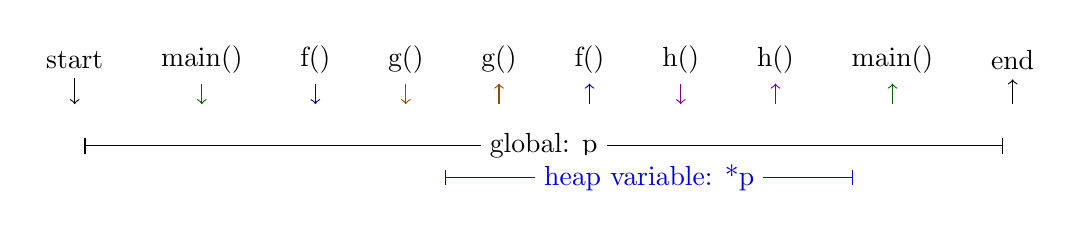
\begin{tikzpicture}
\matrix [ampersand replacement=\&, column sep=5mm, row sep=1mm] {
 \node (bb) {start}; \& \node (bm) {main()}; \& \node (bf) {f()}; \& 
	\node (bg) {g()}; \& \node (cg) {g()}; \& \node (cf) {f()}; \& 
	\node (bh1) {h()}; \& 
	\node (ch1) {h()}; \& \node (cm) {main()}; \& \node (cb) {end}; \\[.5em]
\node (dbb) {}; \& \node (dbm) {}; \& \node (dbf) {}; \& 
	\node (dbg) {}; \& \node (dcg) {}; \& \node (dcf) {}; \& 
	\node (dbh1) {}; \&
	\node (dch1) {}; \& \node (dcm) {}; \& \node (dcb) {}; \\[.2em]
\node (kb) {} ;\& \& \& \& \& \& \& \& \& \node (kc) {}; \\[.2em] 
 \& \& \& \node (yb) {}; \& \& \& \&  \& \node (yc) {}; \& \\
};
\draw [->] (bb) -- (dbb);
\draw [|-|] (kb) -- node [fill=white] {global: p} (kc);
\draw [blue!90!black,|-|] (yb) +(5mm,0) -- node [fill=white] {heap variable: *p} ($(yc) - (5mm,0)$);
\draw [green!40!black,->] (bm) -- (dbm); 
\draw [blue!60!black,->] (bf) -- (dbf); 
\draw [orange!60!black,->] (bg) -- (dbg);  
\draw [orange!60!black,<-] (cg) -- (dcg);
\draw [blue!60!black,<-] (cf) -- (dcf); 
\draw [violet,->] (bh1) -- (dbh1); 
\draw [violet,<-] (ch1) -- (dch1); 
\draw [green!40!black,<-] (cm) -- (dcm);
\draw [<-] (cb) -- (dcb);
\end{tikzpicture}
}
\end{frame}

\defverbatim[colored]\codebasibosC{
\begin{lstlisting}[language={C}]
                                    char *f() {
                                        char a[]="ali";
char *p, *q;                            ....
                                        return a;
p=malloc(10);                       }
q=p;                                ....
...                                 char *p;
free(q);                            p=f();
printf("%s",p);                     printf("%s",p);
\end{lstlisting}}
\subsection{Dangling Reference and Garbage}
\begin{frame}
\frametitle{Dangling Reference}
\begin{itemize}
 \item {\small \structure{dangling reference:} trying to access a variable whose lifetime
 is ended and already deallocated.}
\begin{beamercolorbox}{cexample}
 \codebasibosC
\end{beamercolorbox}
\item {\small both \textsf{p}'s are deallocated or ended lifetime variable, thus dangling
reference}
\item {\small sometimes operating system tolerates dangling references. Sometimes generates
run-time erros like ``protection fault'', ``segmentation fault'' are generated.}
\end{itemize}
 
\end{frame}

\defverbatim[colored]\codebasibosC{
\begin{lstlisting}[language={C}]
                                void f() {
                                    char *p;
char *p, *q;                        p=malloc(10); ...
...                                 return          
p=malloc(10);                   }
p=q;                            ....
...                            f();
\end{lstlisting}}
\begin{frame}
 \frametitle{Garbage variables}
\begin{itemize}
 \item \structure{garbage variables:} The variables with lifetime still continue but there
 is no way to access.
\begin{beamercolorbox}{cexample}
\codebasibosC
\end{beamercolorbox}
\item When the pointer value is lost or lifetime of the pointer is over, heap variable
is unaccessible. (\texttt{*p} in examples)
\end{itemize}
\end{frame}

\begin{frame}
 \frametitle{Garbage collection}
 \begin{itemize}
  \item A solution to dangling reference and garbage problem: PL does management of heap variable deallocation automatically. This is called \structure{garbage collection}. (Java, Lisp, ML, Haskell, most functional languages)
  \item no call like \texttt{free()} or \texttt{delete} exists.
  \item Language runtime needs to:
	\begin{itemize}
		\item Keep a reference counter on each reference, initially 1.
		\item Increment counter on each new assignment
		\item Decrement counter at the end of the reference lifetime
		\item Decrement counter at the overwritten/lost references
		\item Do all these operations recursively on composite values.
		\item When reference count gets 0, deallocate the heap variable
	\end{itemize}
  \end{itemize}
 \end{frame}

\begin{frame}
 \begin{itemize}
  \item Garbage collector deallocates heap variables having a reference count 0.
  \item It usually works in a separate thread, in low priority, works when CPU is idle.
  \item Another but too restrictive solution to garbage: Reference cannot be assigned to a longer lifetime variable.
	local variable references cannot be assigned to global reference/pointer.
 \end{itemize}
\end{frame}

\subsection{Persistent Variable Lifetime}
\begin{frame}
 \frametitle{Persistent variable lifetime}
\begin{itemize}
 \item Variables with lifetime continues after program terminates: file, database, web service object,...
 \item Stored in secondary storage or external process.
 \item Only a few experimental language has transparent persistence. Persistence achieved via IO instructions\\
C files: \texttt{fopen(), fseek(), fread(), fwrite()}
 \item In object oriented languages; \structure{serialization}: Converting object into a binary image
that can be written on disk or sent over the network.
 \item This way objects snapshot can be taken, saved, restored and object continue from where it remains.
\end{itemize}
\end{frame}

\section{Memory Management}
\begin{frame}
\frametitle{Memory Management}
\begin{itemize}
\item Memory manamegement of variables involves architecture, operating system, language runtime and the compiler.
\item A typical OS divides memory in sections (segments):
	\begin{itemize}
	\item Stack section: run time stack
	\item Heap section: heap variables
	\item Data section: global variables
	\item Code section: executable instructions, read only.
	\end{itemize}
\item Global variables are fixed at compile time and they are put in data section.
\item Heap variables are stored in the dynamic data structures in heap section. Heap section grows and shrinks as new variables are allocated and deallocated. 
\item Heap section is maintained by language runtime. For C, it is \texttt{libc}.
\end{itemize}
\end{frame}

\begin{frame}
\frametitle{Local Variables}
\begin{itemize}[<+->]
\item Local variables can have multiple instances alive in case of recursion. 
\item For recursive calls of a function, there should be multiple instances of a variable and compiled code should know where it is depending on the current call state.
\item The solution is to use \structure{run-time stack}. Each function call will introduce an \structure{activation record} to store its local context. It is also called \structure{stack frame, activation frame}.
\item In a typical architecture, \structure{activation record} contains:
	\begin{itemize}
	\item Return address. Address of the next instruction after the caller.
	\item Parameter values.
	\item A reserved area for local variables.
	\end{itemize}
\end{itemize}
\end{frame}

\begin{frame}[fragile]
\begin{columns}
\begin{column}{.4\textwidth}
\begin{beamercolorbox}{cexample}\small
\begin{lstlisting}[tabsize=4,numbers=left]
int f(short a, int b) {
	char tmp[10];
	...
	return a+b;
}
int g(int x) {
	int tmp, p;
	...
	tmp = f(x, x+1);
	...
	return tmp+p;
}
int main() {
	return g(4);
}
\end{lstlisting}
\end{beamercolorbox}
\end{column}
\begin{column}{.6\textwidth}
\tiny
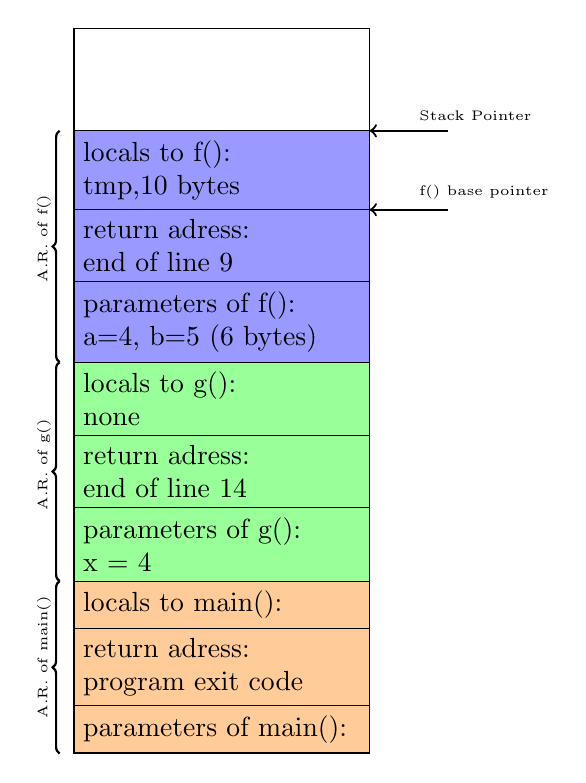
\begin{tikzpicture}
   [stack/.style={rectangle split, rectangle split parts=#1,draw,
	 text width=10em}]
\node [stack=10, rectangle split part fill={white,blue!40!white,blue!40!white,blue!40!white,
		green!40!white, green!40!white, green!40!white,
		orange!40!white, orange!40!white, orange!40!white}] (stk) {
\nodepart{one} \rule{0pt}{3em}
\nodepart{two} locals to f():\\
               tmp,10 bytes
\nodepart{three} return adress:\\
				end of line 9
\nodepart{four} parameters of f():\\
				a=4, b=5 (6 bytes)
\nodepart{five} locals to g():\\
				none
\nodepart{six} return adress:\\
				end of line 14
\nodepart{seven} parameters of g():\\
				x = 4
\nodepart{eight} locals to main():\\
\nodepart{nine} return adress:\\
			   program exit code
\nodepart{ten} parameters of main():\\
};
\draw [decorate,thick,decoration={brace,mirror,raise=5pt}] (stk.text split west) to (stk.four split west); 
\draw [decorate,thick,decoration={brace,mirror,raise=5pt}] (stk.four split west) to (stk.seven split west); 
\draw [decorate,thick,decoration={brace,mirror,raise=5pt}] (stk.seven split west) to (stk.south west); 
\node [left=of stk.three,rotate=90,anchor=center,yshift=-5mm] {\tiny A.R. of f()};
\node [left=of stk.six,rotate=90,anchor=center,yshift=-5mm] {\tiny A.R. of g()};
\node [left=of stk.nine,rotate=90,anchor=center,yshift=-5mm] {\tiny A.R. of main()};
\draw [->,thick] ($(stk.text split east) + (1cm,0)$) {} -- node [above,anchor=south west] {\tiny Stack Pointer}
		(stk.text split east);
\draw [->,thick] ($(stk.two split east) + (1cm,0)$) {} -- node [above,anchor=south west] {\tiny f() base pointer}
		(stk.two split east);
\end{tikzpicture} 
\end{column}
\end{columns}
\end{frame}

\begin{frame}
\frametitle{Function Call}
\setbeamerfont{itemize/enumerate body}{size={\fontsize{11}{12}}}
\setbeamerfont{enumerate item}{size={\fontsize{10}{11}}}
\setbeamerfont{itemize/enumerate subbody}{size={\fontsize{10}{11}}}
\setbeamerfont{enumerate subitem}{size={\fontsize{9}{10}}}
\begin{itemize}
\item Caller side:
	\begin{enumerate}
	\item Push parameters
	\item Push return address and jump to function code start\\
		(usually a single CPU instruction like \lstinline!callq!)
	\end{enumerate}
\item Function entry:
	\begin{enumerate}
	\item Set base pointer to current stack pointer
	\item Advance stack pointer to size of local variables
	\end{enumerate}
\item Function body can access all local variables relative to base pointer\
\item Function return:
	\begin{enumerate}
	\item Set stack pointer to base pointer
	\item Pop return address and jump to return address\\
		(single CPU instruction like \lstinline!retq!)
	\end{enumerate}
\item Caller side after return:
	\begin{enumerate}
	\item Recover stack pointer (remove parameters on stack)
	\item Get and use return value if exists (typically from a register)
	\end{enumerate}
\end{itemize}
\end{frame}

\begin{frame}[fragile]
\begin{itemize}
\item All locals and parameters
	have the same offset from base pointer
\item Recursive calls execute same instructions
\end{itemize}
\begin{columns}[b]
\begin{column}{.4\textwidth}
\begin{beamercolorbox}{cexample}\small
\begin{lstlisting}[tabsize=4,numbers=left]
int h(int n) {
	int tmp;
	if (n <= 1) return 0;
    else {
		tmp = h(n-1);
		return n+tmp;
	}
}
int main() {
	printf("%d\n", h(2));
	return 0;
}
\end{lstlisting}
\end{beamercolorbox}
\end{column}
\begin{column}{.6\textwidth}
{\tiny
\only<1-1>{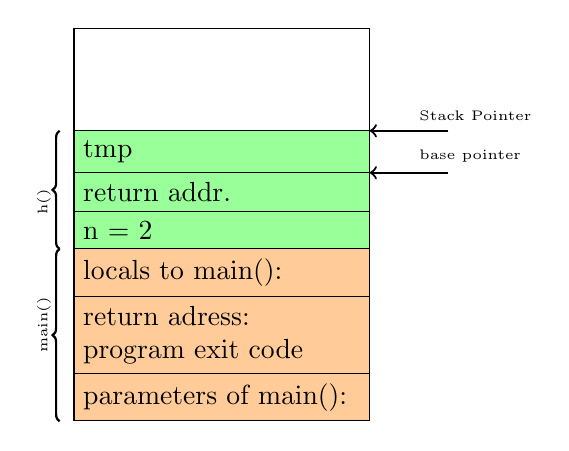
\begin{tikzpicture}
   [stack/.style={rectangle split, rectangle split parts=7,draw,
	 text width=10em},
	scolor/.style={rectangle split part fill={white,
 			green!40!white, green!40!white, green!40!white,
			orange!40!white, orange!40!white, orange!40!white}}]
\node [stack,scolor] (stk) {
\nodepart{one} \rule{0pt}{3em}
\nodepart{two} tmp
\nodepart{three} return addr.
\nodepart{four} n = 2
\nodepart{five} locals to main():\\
\nodepart{six} return adress:\\
			   program exit code
\nodepart{seven} parameters of main():\\
};
\draw [decorate,thick,decoration={brace,mirror,raise=5pt}] (stk.text split west) to (stk.four split west); 
\draw [decorate,thick,decoration={brace,mirror,raise=5pt}] (stk.four split west) to (stk.south west); 
\node [left=of stk.three,rotate=90,anchor=center,yshift=-5mm] {\tiny h()};
\node [left=of stk.six,rotate=90,anchor=center,yshift=-5mm] {\tiny main()};
\draw [->,thick] ($(stk.text split east) + (1cm,0)$) {} -- node [above,anchor=south west] {\tiny Stack Pointer}
		(stk.text split east);
\draw [->,thick] ($(stk.two split east) + (1cm,0)$) {} -- node [above,anchor=south west] {\tiny base pointer}
		(stk.two split east);
\end{tikzpicture}\\}%
\only<2-2>{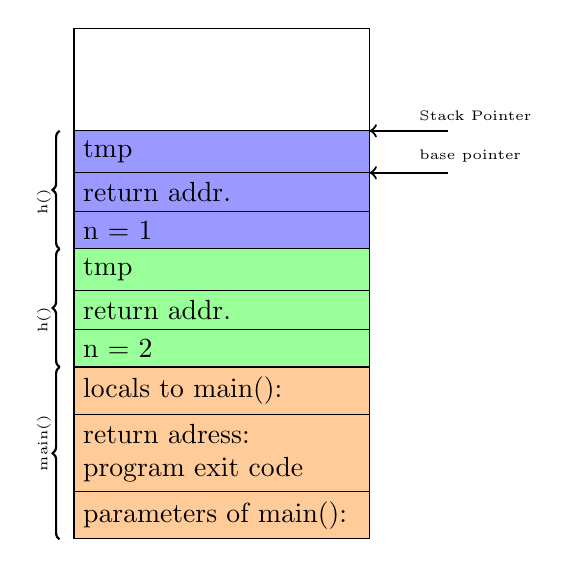
\begin{tikzpicture}
   [stack/.style={rectangle split, rectangle split parts=10,draw,
	 text width=10em},
	scolor/.style={rectangle split part fill={white,blue!40!white,blue!40!white,blue!40!white,%
							green!40!white, green!40!white, green!40!white,%
							orange!40!white, orange!40!white, orange!40!white}}]

\node [stack,scolor] (stk) {
\nodepart{one} \rule{0pt}{3em}
\nodepart{two} tmp
\nodepart{three} return addr.
\nodepart{four} n = 1
\nodepart{five} tmp
\nodepart{six} return addr.
\nodepart{seven} n = 2
\nodepart{eight} locals to main():\\
\nodepart{nine} return adress:\\
			   program exit code
\nodepart{ten} parameters of main():\\
};
\draw [decorate,thick,decoration={brace,mirror,raise=5pt}] (stk.text split west) to (stk.four split west); 
\draw [decorate,thick,decoration={brace,mirror,raise=5pt}] (stk.four split west) to (stk.seven split west); 
\draw [decorate,thick,decoration={brace,mirror,raise=5pt}] (stk.seven split west) to (stk.south west); 
\node [left=of stk.three,rotate=90,anchor=center,yshift=-5mm] {\tiny h()};
\node [left=of stk.six,rotate=90,anchor=center,yshift=-5mm] {\tiny h()};
\node [left=of stk.nine,rotate=90,anchor=center,yshift=-5mm] {\tiny main()};
\draw [->,thick] ($(stk.text split east) + (1cm,0)$) {} -- node [above,anchor=south west] {\tiny Stack Pointer}
		(stk.text split east);
\draw [->,thick] ($(stk.two split east) + (1cm,0)$) {} -- node [above,anchor=south west] {\tiny base pointer}
		(stk.two split east);
\end{tikzpicture}\\}}
\end{column}
\end{columns}
\end{frame}

\begin{frame}[fragile]
\begin{itemize}
\item Order of values in the activation record may differ for different languages
\item Registers are used for passing primitive value parameters instead of stack
\item Garbage collecting languages keep references on stack with actual variables on heap
\item Languages returning nested functions as first order values require more complicated mechanisms\\
\begin{beamercolorbox}{pexample}
{\small
\begin{lstlisting}[language=Python]
def multiplier(a):
	def f(x):
		return a*x
	return f

twice = multiplier(2)
# multiplier/a is not alive anymore but twice=f is using it
print(twice(14))
\end{lstlisting}
}
\end{beamercolorbox}
\end{itemize}
\end{frame}

\section{Commands}
\begin{frame}
 \frametitle{Commands}
 \structure{Expression:} program segment with a value.\\
 \structure{Statement:} program segment without a value, but alters the state. Input, output, variable assignment, iteration...
\begin{enumerate}
 \item Assignment
 \item Procedure call
 \item Block commands
 \item Conditional commands
 \item Iterative commands
\end{enumerate}
\end{frame}

\subsection{Assignment}
\begin{frame}
 \frametitle{Assignment}
\begin{itemize}
 \item C: ``\texttt{Var = Expr;}'', Pascal ``\texttt{Var := Expr;}''.
 \item Evaluates RHS expression and sets the value of the variable at RHS
 \item \texttt{ x = x + 1} . LHS \texttt{x} is a variable reference (l-value), RHS is the value
 \item  \structure{multiple assignment:} \texttt{ x=y=z=0;}
 \item \structure{parallel assignment:} (Perl, PHP) \texttt{ (\$a,\$b) = (\$b, \$a);} \\
	\texttt{(\$name, \$surname, \$no) = ("Onur","Şehitoğlu",55717);} \\
	Assignment: ``reference aggregate'' $\rightarrow$ ``value aggregate''
 \item \structure{assignment with operator:} \texttt{ x += 3; x *= 2; }
\end{itemize}
\end{frame}

\subsection{Procedure Call}
\begin{frame}
 \frametitle{Procedure call}
\begin{itemize}
 \item \structure{Procedure:} user defined commands. Pascal: \structure{procedure}, 
	C: \structure{function returning void}
 \item \texttt{void {\em functname\/}({\em param1\/}, {\em param2\/}, ..., {\em paramn\/})}
 \item Usage is similar to functions but call is in a statement position (on a separate line of
	program)
\end{itemize}
\end{frame}

\subsection{Block commands}
\begin{frame}
 \frametitle{Block commands}
\begin{itemize}
 \item Composition of a block from multiple statements
 \item \structure{Sequential commands:} \texttt{ \{ C$_1$ ; C$_2$; ... ; C$_n$ \}} \\
A command is executed, after it finishes the next command is executed,...     
\item  Commands enclosed in a block behaves like single command:``if'' blocks, loop bodies,... 
\item \structure{Collateral commands:}
\texttt{ \{  C$_1$, C$_2$, ... , C$_n$ \}} \alert{\scriptsize (not C `,')!}\\ Commands can be executed in any order.
\item The order of execution is non-deterministic. Compiler or optimizer can choose any order. If commands are independent, effectively deterministic:\\`\texttt{y=3 , x=x+1 ;}' vs `\texttt{x=3, x=x+1 ;}'
\item Can be executed in parallel.
\end{itemize}
\end{frame}

\defverbatim[colored]\codethreadC{
\begin{lstlisting}[language={C}]
void producer(...) {....}
void collectgarbage(...) {....}
void consumer(...) {....}
int main() {
	...
	pthread_create(tid1,NULL,producer,NULL);
	pthread_create(tid2,NULL,collectgarbage,NULL);
	pthread_create(tid3,NULL,consumer,NULL);
	...
}
\end{lstlisting}}

\begin{frame}
\begin{itemize}
  \item \structure{Concurrent commands:} concurrent paradigm languages:\\
\texttt{ \{  C$_1$ $\mid$ C$_2$ $\mid$ ... $\mid$ C$_n$ \}}
  \item All commands start concurrently in parallel. Block finishes when the last active command finishes.
  \item Real parallelism in multi-core/multi-processor machines.
  \item Transparently handled by only a few languages. Thread libraries required in languages like Java, C, C++.
\begin{beamercolorbox}{cexample}
 \codethreadC
\end{beamercolorbox}

\end{itemize}
\end{frame}

\subsection{Conditional commands}
\begin{frame}
\frametitle{Conditional commands}
\begin{itemize}
 \item Commands to choose between alternative commands based on a condition
 \item in C : \texttt{if ({\em cond\/}) $C_1$ else $C_2$ ; } \\
	\texttt{\small switch ({\em value\/}) 
		  \{ case $L_1$ : $C_1$ ;  case $L_2$ : $C_2$ ; ...\}} 
 \item \texttt{if} commands can be nested for multi-conditioned selection.
 \item \texttt{switch} like commands chooses  statements based on a value\\ {\scriptsize
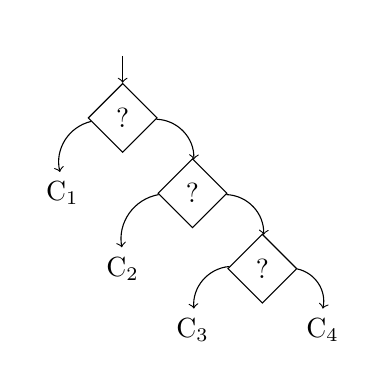
\begin{tikzpicture}
\matrix [ampersand replacement=\&,row sep=2pt] {
	\& \node (basla) {}; \\[.8em]
	\& \node [diamond,draw] (k1) {?}; \\
\node (K1) {C$_1$}; \&               \& \node [diamond,draw] (k2) {?}; \\
				    \& \node (K2) {C$_2$}; \&               \& \node [diamond,draw] (k3) {?}; \\
				    \&				\& \node (K3) {C$_3$}; \&               \& \node (K4) {C$_4$}; \\
};
\draw [->] (basla) -- (k1) ;
\draw [->] (k1) to [bend left=45] (k2);
\draw [->] (k1) to [bend right=45]  (K1);
\draw [->] (k2) to [bend right=45]  (K2);
\draw [->] (k2) to [bend left=45]  (k3);
\draw [->] (k3) to [bend right=45]  (K3);
\draw [->] (k3) to [bend left=45]  (K4);
\end{tikzpicture}
}
%\begin{tabular}{ccccc}
%      & \rnode{basla}{\rule{0pt}{1em}}\\
%      & \rnode{k1}{\psdiabox[framearc=0.6]{?}}  \\
%\rnode{K1}{C$_1$} &     & \rnode{k2}{\psdiabox{?}} \\
%      &  \rnode{K2}{C$_2$} &      &     \rnode{k3}{\psdiabox{?}} \\
%      &           &   \rnode{K3}{C$_3$} &     & \rnode{K4}{C$_4$} \\
%\end{tabular}
%\ncline{->}{basla}{k1}
%\ncdiag[angleA=180,angleB=90,linearc=.5]{->}{k1}{
%\ncdiag[angleA=0,angleB=90,linearc=.2]{->}{k1}{k2}
%\ncdiag[angleA=180,angleB=90,linearc=.5]{->}{k2}{K2}
%\ncdiag[angleA=0,angleB=90,linearc=.2]{->}{k2}{k3}
%\ncdiag[angleA=180,angleB=90,linearc=.2]{->}{k3}{K3}
%\ncdiag[angleA=0,angleB=90,linearc=.2]{->}{k3}{K4}
%}
{\scriptsize
\begin{tikzpicture}
\matrix [ampersand replacement=\&,column sep=1mm] {
	\& \&\node (basla) {}; \\[.8em]
	\& \& \node [diamond,aspect=1.5,draw] (k1) {\tiny Value}; \\[2em]
\node (K1) {C$_1$}; \& \node (K2) {C$_2$}; \&  \& \node (K3) {C$_3$};  \& \node (K4) {C$_4$}; \\[4em]
\node {} ;\\
};
\draw [->] (basla) -- (k1) ;
\draw [->] (k1) .. controls +(180:15mm) and +(90:5mm) .. node [fill=white] {\tiny L$_1$} (K1);
\draw [->] (k1) .. controls +(200:10mm) and +(90:5mm) .. node [fill=white] {\tiny L$_2$}   (K2);
\draw [->] (k1) .. controls +(-20:10mm) and +(90:5mm) .. node [fill=white] {\tiny L$_3$}  (K3);
\draw [->] (k1) .. controls +(0:15mm) and +(90:5mm) .. node [fill=white] {\tiny L$_4$} (K4);
\end{tikzpicture}}
\end{itemize}
\end{frame}
%\begin{tabular}{cccc}
%      & \rnode{swbasla}{\rule{0pt}{1em}}\\
%      & \rnode{swsec}{\psdiabox[framearc=0.6]{Val}}  \\[3.5em]
%\rnode{sK1}{C$_1$} &    \rnode{sK2}{C$_2$} & \rnode{sK3}{C$_3$} 
%&    \rnode{sK4}{C$_4$} \\
%\end{tabular}
%\ncline{->}{swbasla}{swsec}
%\ncdiag[angleA=180,angleB=90,linearc=.2]{->}{swsec}{sK1}
%\mput*{L$_1$}
%\ncline{->}{swsec}{sK2}
%\mput*{L$_2$}
%\ncdiag[angleA=300,angleB=90,linearc=.2]{->}{swsec}{sK3}
%\mput*{L$_3$}
%\ncdiag[angleA=0,angleB=90,linearc=.2]{->}{swsec}{sK4}
%\mput*{L$_4$}
%

\begin{frame}
 \begin{itemize}
  \item \structure{non-deterministic conditionals:} conditions are evaluated in collaterally and commands
	are executed if condition holds.
  \item hyphotetically:\\ \texttt{\small if ({\em cond$_1$\/}) $C_1$ or if ({\em cond$_2$\/}) $C_2$ or if ({\em cond$_3$\/}) $C_3$  ; } \\[1em]
	\texttt{\small switch ({\em val\/}) \{ \\ 
	\hspace*{3em}case {\em L$_1$}: $C_1$ $\mid$ case {\em L$_2$}: $C_2$ $\mid$ case {\em L$_3$}: $C_3$ \}}
  \item Tests can run concurrently. First test evaluating to \lstinline!True! wins. Others discarded.\\
{\scriptsize
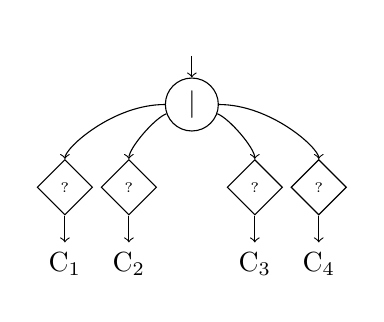
\begin{tikzpicture}
\matrix [ampersand replacement=\&,column sep=1mm] {
	\& \&\node (basla) {}; \\[.8em]
	\& \& \node [circle,draw] (k1) {$\mid$}; \\[1em]
\node [diamond,draw](K1) {\tiny ?}; \& \node [diamond,draw](K2) {\tiny ?}; \&  \& \node [diamond,draw](K3) {\tiny ?};  \& \node [diamond,draw](K4) {\tiny ?}; \\[1em]
\node (CK1) {C$_1$}; \& \node (CK2) {C$_2$}; \&  \& \node (CK3) {C$_3$};  \& \node (CK4) {C$_4$}; \\
};
\draw [->] (basla) -- (k1) ;
\draw [->] (k1) .. controls +(180:10mm) and +(90:5mm) ..  (K1);
\draw [->] (k1) .. controls +(200:5mm) and +(90:5mm) ..  (K2);
\draw [->] (k1) .. controls +(-20:5mm) and +(90:5mm) ..  (K3);
\draw [->] (k1) .. controls +(0:10mm) and +(90:5mm) ..  (K4);
\draw [->] (K1) -- (CK1);
\draw [->] (K2) -- (CK2);
\draw [->] (K3) -- (CK3);
\draw [->] (K4) -- (CK4);
\end{tikzpicture}
}
%\begin{tabular}{cccc}
%      & \rnode{pibasla}{\rule{0pt}{1em}}\\
%      & \rnode{pik1}{\pscirclebox{\rule{0pt}{1em}$\mid$}} \\[1.5em]
%\rnode{piK1}{\psdiabox[framearc=0.6]{?}}  &
%\rnode{piK2}{\psdiabox[framearc=0.6]{?}}  &
%\rnode{piK3}{\psdiabox[framearc=0.6]{?}}  &
%\rnode{piK4}{\psdiabox[framearc=0.6]{?}}  \\[1.5em]
%\rnode{picK1}{C$_1$} & \rnode{picK2}{C$_2$} & 
%	\rnode{picK3}{C$_3$} & \rnode{picK4}{C$_4$} \\
%\end{tabular}
%\ncline{->}{pibasla}{pik1}
%\ncdiag[angleA=180,angleB=90,linearc=.2]{->}{pik1}{piK1}
%\ncline{->}{pik1}{piK2}
%\ncline{->}{pik1}{piK3}
%\ncdiag[angleA=0,angleB=90,linearc=.2]{->}{pik1}{piK4}
%\ncline{->}{piK1}{picK1}
%\ncline{->}{piK2}{picK2}
%\ncline{->}{piK3}{picK3}
%\ncline{->}{piK4}{picK4}
 \end{itemize}

\end{frame}


\subsection{Iterative statements}
\begin{frame}
\frametitle{Iterative statements}
\begin{itemize}[<+->]
 \item Repeating same command or command block multiple times possibly with different data or state. Loop commands.
 \item Loop classification: minimum number of iteration: 0 or 1.
\begin{columns}
 \begin{column}{.5\linewidth}
C: \texttt{while (...) \{ ... \}}\\
   {\scriptsize
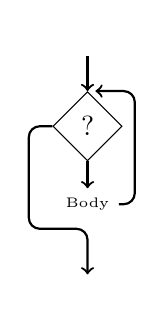
\begin{tikzpicture}
\matrix [ampersand replacement=\&] {
      \& \node (Dbasla){} ; \\[1.3em]
      \& \node [diamond,draw] (Dk){?}; \\[1em]
      \& \node (DYK){\tiny Body}    ; \\[2em]
      \& \node (DBit){}     ;\\
};
\draw [->,thick] (Dbasla) -- (Dk);
\draw [->,thick] (Dk) -- (DYK);
\draw [->,thick,rounded corners=4pt] (DYK) -- +(6mm,0) -- ($(Dk.north) + (6mm,0)$) -- ($(Dk.north) + (1mm,0)$);
\draw [->,thick,rounded corners=4pt] (Dk.west) -- +(-3mm,0) -- ($(Dk.west) - (3mm,-2em) + (DBit) - (Dk)$) 
		-- ($(DBit) + (0,2em)$) --  (DBit);
\end{tikzpicture}
}
 \end{column}
\begin{column}{.5\linewidth}
 C: \texttt{do \{...\} while (...);}\\
   {\scriptsize
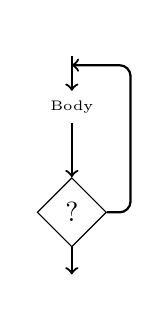
\begin{tikzpicture}
\matrix [ampersand replacement=\&] {
      \& \node (Dbasla){} ; \\[1.3em]
      \& \node (DYK){\tiny Body}    ; \\[2em]
      \& \node [diamond,draw] (Dk){?}; \\[1em]
      \& \node (DBit){}     ;\\
};
\draw [->,thick] (Dbasla) -- (DYK);
\draw [->,thick] (DYK) -- (Dk);
\draw [->,thick,rounded corners=4pt] (Dk.east) -- +(3mm,0) -- ($(Dk.east) + (3mm,1.5em) - (Dk) + (DYK)$) 
		-- ($(DYK) + (0,1.5em)$) ;
\draw [->,thick] (Dk) -- (DBit);
\end{tikzpicture}
%\begin{tabular}{cc}
%      & \rnode{Dbasla}{}\\[1em]
%      & \rnode{DYK}{IC}      \\[2em]
%      & \rnode{Dk}{\psdiabox{?}}  \\
%      & \rnode{DBit}{}      \\
%\end{tabular}
%\ncline{->}{Dbasla}{DYK}
%\ncline{->}{DYK}{Dk}
%\ncline{->}{Dk}{DBit}
%\ncbar[angleA=0,angleB=-90,linearc=.2]{->}{Dk}{Dbasla}
%\ncbar[angleA=180,angleB=90,arm=.2,linearc=.3]{->}{Dk}{DDon}
%\ncline{->}{DDon}{DBit}
} 
 \end{column}
\end{columns}
\end{itemize}
\end{frame}


\defverbatim[colored]\codelistePhp{
\begin{lstlisting}[language={PHP}]
$colors=array('yellow','blue','green','red','white');
foreach ($colors as $i) {
    print $i," is a color","\n";
}
\end{lstlisting}}
\begin{frame}
\begin{itemize}
 \item Definite vs indefinite loops
 \item \structure{Indefinite iteration:} Number of iterations of the loop is not known until loop finishes
\item C loops are indefinite iteration loops.
\item \structure{Definite iteration:} Number of iterations is fixed when loop started.
\item Pascal \texttt{for} loop is a definite iteration loop. \\
	\texttt{ for i:= k to m  do begin .... end;}  has $(m-k+1)$ iterations.\\
	Pascal forbids update of the loop index variable.
\item List and set based iterations: PHP, Perl, Python, Shell
\begin{beamercolorbox}{oexample}
\codelistePhp
\end{beamercolorbox}
\end{itemize}
\end{frame}

\section{Summary}
\begin{frame}
 \frametitle{Summary}
\begin{itemize}
 \item Variables with storage
 \item Variable update
 \item Lifetime: global, local, heap, persistent
 \item Commands
\end{itemize}

\end{frame}





\end{document}
